\documentclass[11pt,a4paper]{article}
\usepackage[margin=2.3cm]{geometry}
\usepackage{fontspec}
\usepackage{amsmath,amssymb}
\usepackage{graphicx,booktabs,caption,subcaption}
\usepackage[round,authoryear]{natbib}
\usepackage{xcolor,tikz}
\usetikzlibrary{positioning,arrows.meta,calc}
\usepackage[colorlinks=true,linkcolor=blue!50!black,citecolor=blue!50!black,urlcolor=blue!50!black]{hyperref}
\usepackage{eso-pic}
\graphicspath{{../analysis/out/figs/}}
\input{../analysis/out/stats.tex}
% analyses that need fields absent from older data files fall back to n/a
\providecommand{\HoneBoundary}{n/a}
\providecommand{\NSchool}{0}
\providecommand{\CheckPractice}{n/a}
\providecommand{\HtwoBoundaryAsTap}{n/a}
\providecommand{\CheckEffortAsTap}{n/a}
\providecommand{\HtwoAsTapDL}{n/a}
\providecommand{\HtwoAsTapUnfiltered}{n/a}
\providecommand{\HtwoAsTapStrict}{n/a}
\providecommand{\HtwoCostAsTapAll}{n/a}
\providecommand{\CheckEffortAsNone}{n/a}

% every page carries a warning while the numbers come from simulated data
\ifsimulated
  \AddToShipoutPictureBG{\AtPageCenter{\makebox(0,0){\rotatebox{40}{\textcolor{red!25}{\fontsize{56}{56}\selectfont SIMULATED DATA}}}}}
\fi
\newcommand{\todo}[1]{\textcolor{red}{[#1]}}

\title{\textbf{Does the Mind's Compression Code Need Words?}\\[4pt]
\large Language-of-thought complexity, inner speech, and memory for spatial sequences}
\author{\small
\begin{tabular}{lll}
Gokul VKS & 2401020094 & B.Tech (Computer Science \& Data Science)\\
Mahir Abdhullah & 2401010256 & B.Tech (Computer Science \& AI)\\
Mohan Kumar C R & 2401010282 & B.Tech (Computer Science \& AI)\\
Shrihari K N & 2401010448 & B.Tech (Computer Science \& AI)\\
Gangeli Devanand Siddhardha & 2402110008 & BBA
\end{tabular}\\[6pt]
\small Cognitive Psychology: Cognitive Task Design Project\\
\small Task: \url{https://constellations-task.vercel.app}\\
\small Code: \url{https://github.com/mahir-m01/constellations}}
\date{November 2026}

\begin{document}
\maketitle

\begin{abstract}
\noindent People remember structured sequences far better than random ones, and the advantage is predicted by the length of a
sequence's shortest description in a ``language of thought'' (LoT). Whether this internal code relies on natural language is a
live question \citep{fedorenko2024language}. We built \emph{Constellations}, a new browser-based task in which participants
watch eight stars on an octagon light up one at a time and then click them in the same order. Each participant recalled four
of 14 eight-item sequences spanning the full range of LoT complexity ($K = 5$--16) in three blocks: (a) no concurrent task,
(b) repeating ``the'' aloud (articulatory suppression, checked by microphone loudness) and (c) tapping a key at a similar
rate (a matched non-verbal control). If the compression code depends on inner speech, suppression, but not tapping, should
flatten the complexity effect. In total, \NAll{} people completed the task (age \AgeMin--\AgeMax, median \AgeMedian). Recall fell steeply
with complexity (\AccKFive{} of positions correct for the simplest sequence, \AccKSixteen{} for the most complex), and the
compression benefit with no concurrent task was large and reliable, \HoneStat. Only \NFinal{} participants performed both
concurrent tasks reliably, mostly because tapping lapsed. In that compliant sample suppression did not flatten the
complexity effect (\HtwoAsTap); with all \NAll{} participants and no compliance filter there was a non-significant trend in the
predicted direction (\HtwoAsTapUnfiltered). Recall was not related to age, gender, mathematical training, sleep, gaming or
inner-speech habits. The study replicates LoT compression in a new recall format; whether compression needs inner speech
remains open and needs a larger sample with better-enforced tapping.
\end{abstract}

% =====================================================================
\section{Introduction}

\subsection{Memory as compression}
The capacity of short-term memory is famously limited \citep{miller1956magical,cowan2001magical}, yet that limit is not fixed:
people remember more when the material contains regularities they can exploit. Simplicity, in the information-theoretic sense of
a short description, has been proposed as a unifying principle in cognitive science \citep{chater2003simplicity}. The difficulty of
learning a Boolean concept tracks the length of its minimal formula \citep{feldman2000minimization}, short-term memory span is
better described by the compressibility of the material than by a fixed number of items \citep{mathy2012magic}, and visual working
memory stores more items when their co-occurrence statistics allow a compressed code \citep{brady2009compression}.

\subsection{A language of thought for geometry and sequences}
Dehaene and colleagues have made this idea precise for sequences. In the octagon paradigm \citep{amalric2017language},
participants watch a sequence of locations on the vertices of a regular octagon. Sequences are described in a minimal formal
language with geometric primitives (rotations, axial and point symmetries) and a repetition operator that can be nested; each
sequence's \emph{LoT complexity} is the length of its shortest program in this language. Adults and preschool children
encoded sequences in ways predicted by minimal description length \citep{amalric2017language}. The same approach explains
memory for binary auditory and visual sequences better than statistical-learning alternatives \citep{planton2021theory},
predicts working-memory performance and anticipatory brain signals for spatial sequences \citep{alroumi2021mental}, and
correlates with activity in dorsal inferior prefrontal cortex \citep{wang2019representation}. The authors argue that such
``mental programs'' reflect a symbolic, compositional code that may be uniquely human \citep{dehaene2022symbols}, and the
framework extends to geometric shapes \citep{sablemeyer2022language}. For binary auditory sequences, brain responses
that scale with LoT complexity overlap with a mathematical-calculation localiser and only minimally with the language
network \citep{alroumi2023brain}, and children and adults, unlike macaques, spontaneously extract such relational rules from
spatial sequences \citep{zhang2022working}.

\subsection{Is the language of thought a language?}
A natural objection is that the ``language'' of thought may simply be language: participants could verbally recode a sequence
(``a square, then the same square rotated''), and the compression advantage would then be a verbal-recoding advantage. Two
literatures point in opposite directions. On one side, the brain's language network is largely dissociable from the networks
supporting mathematics, logic and other forms of complex reasoning \citep{fedorenko2016language,fedorenko2024language}: patients
with severe agrammatic aphasia can still solve mathematical problems \citep{varley2005agrammatic}, deductive inference recruits
regions outside the language network \citep{monti2009boundaries}, and advanced mathematics in professional mathematicians
activates a network distinct from language areas \citep{amalric2016origins}. On the other side, inner speech is a pervasive
feature of human cognition \citep{aldersonday2015inner}; preventing it with articulatory suppression impairs cognitive control
in task switching \citep{emerson2003role}; verbal labels can modulate perception and categorisation
\citep{lupyan2012linguistically}, and aphasic naming deficits predict selective impairments on rule-like categorisation
\citep{lupyan2013linking}; and people who report little inner speech differ on some verbal tasks
\citep{nedergaard2024not}. Individual differences in habitual verbal thinking can be measured with the Internal Representations
Questionnaire \citep{roebuck2020internal}.

\subsection{What is already known, and what is not}
Spatial sequence memory is largely immune to articulatory suppression: in the Corsi task, suppression during encoding did not
impair forward recall whereas matrix tapping did \citep{vandierendonck2004working}. Structured paths keep their advantage under
concurrent visuospatial suppression \citep{kemps2001complexity}; the recall advantage for symmetric configurations does not
interact with articulatory suppression \citep{rossiarnaud2006symmetry}; spatial path complexity affects verbal serial recall
even under suppression \citep{allan2017right}; and the benefit of a familiar spatial layout for verbal recall survives
suppression but is abolished by spatial tapping \citep{allen2024maintaining}. Regular, single-key tapping, in contrast, leaves
verbal serial recall intact \citep{larsen2003disruption}. Closest to the present question, a recent preprint showed that an
order-based LoT model predicts 12-item spatial serial recall almost perfectly ($r = .96$) and that inter-click intervals slow
at the boundaries of the inferred mental program \citep{tabbane2026humans}. That study randomised geometry, however, and
included neither a concurrent task nor measures of inner speech. Strategy work shows that people do spontaneously label
spatial memoranda with words \citep{seabra2025verbal} and differ strongly in non-verbal (overt versus covert) rehearsal
strategies \citep{desardenberg2024inter}.

\subsection{The present study}
No study to our knowledge has crossed \emph{graded geometric LoT complexity} with articulatory suppression and a matched
non-verbal control, or related the result to individual differences in inner speech. Articulatory suppression (repeating an
irrelevant word aloud) occupies the articulatory rehearsal process of the phonological loop
\citep{baddeley1984exploring,baddeley2012working}; rhythmic single-key tapping at the same rate controls for the general cost
of doing two things at once. We note the limit of this logic at the outset: suppression blocks \emph{subvocal verbal recoding},
not the entire language network, so our question is whether compression depends on inner speech, not whether it depends on
every aspect of language \citep{fedorenko2024language}. Table~\ref{tab:predictions} summarises what each account predicts.

\paragraph{Research question.} Does the memory advantage for compressible (low-complexity) spatial sequences depend on inner
speech, and how does sequence memory vary across conditions and across individuals (age, gender, field of study, mathematical
training and habitual inner speech)?

\begin{table}[t]\centering\small
\caption{Predictions of competing accounts. Slope = accuracy lost per unit of LoT complexity (the compression benefit).}
\label{tab:predictions}
\begin{tabular}{p{3.6cm}p{2.3cm}p{2.5cm}p{2.9cm}p{2.6cm}}\toprule
Account & Recall vs.\ complexity & Suppression vs.\ tapping & Suppression $\times$ complexity & Inner-speech moderation \\ \midrule
Non-linguistic geometric LoT \citep{dehaene2022symbols,fedorenko2024language} & Strong decline & Equal costs & Slope unchanged & None \\
Verbal recoding / label feedback \citep{lupyan2012linguistically,emerson2003role} & Decline & Suppression costlier & Slope flattened (simple sequences lose their advantage) & Larger flattening with more inner speech \\
Visuospatial structure \citep{kemps2001complexity,allen2024maintaining} & Decline & Equal costs (non-spatial tapping) & Unchanged or steeper & None \\
Pluralistic strategies \citep{nedergaard2024not,seabra2025verbal} & Decline & Depends on the person & Flattened only for habitual verbalisers & Positive \\ \bottomrule
\end{tabular}
\end{table}

\paragraph{Hypotheses.}
\textbf{H1} (compression): recall accuracy decreases with LoT complexity, and LoT complexity predicts accuracy better than
simpler descriptors (Lempel--Ziv complexity, step entropy, number of step runs, path length, crossings).
\textbf{H1b} (program boundaries): inter-click intervals are longer when entering a new sub-program (e.g.\ the second square of
\emph{2squares}) than within one \citep{tabbane2026humans}.
\textbf{H2a} (non-linguistic code): articulatory suppression and tapping impose similar overall costs, and the complexity slope
is the same under suppression as under tapping.
\textbf{H2b} (verbal recoding): suppression \emph{selectively} flattens the complexity slope, because simple sequences lose the
advantage of a short verbal description.
\textbf{H3} (exploratory): the suppression-specific flattening is larger for people with more habitual inner speech; the
compression benefit is larger with more mathematical training; and suppression reduces metacognitive sensitivity
(confidence--accuracy correspondence) relative to tapping, if inner speech supports self-monitoring.

% =====================================================================
\section{Method}

\subsection{Participants}
\NAll{} people completed the full task between 25 and 28 November 2026 (\NFemale{} female, \NMale{} male, one preferred not to say;
age $M = \AgeMean$, $SD = \AgeSD$, median \AgeMedian, range \AgeMin--\AgeMax). Most were undergraduates (19 college students,
13 of them in their third year); \NSchool{} were school students and one was not studying. \NStem{} studied a science,
technology or health subject and \NNonStem{} commerce or arts. Participants were recruited by the group members and took part online on their own device, using a laptop or desktop
with a trackpad or mouse (15) or a touchscreen (8); the median session lasted
\DurationMedian{} minutes. Every session was complete (all 15 trials), each came from a different email address, and the
three test sessions run by the authors were excluded. Age, course, gender and email were collected from everyone, as required.

\paragraph{Ethics.} Participants gave informed consent on the first screen, which explained the task, the microphone check
(loudness only, no recording) and how the data would be used. \NMinors{} participants were under 18 (aged 14--15); a parent or
guardian agreed to their participation. Email addresses were collected only to identify duplicate sessions, were never used in
any analysis, and all results are reported anonymously by participant code. With all $N = \NAll$ participants a two-sided paired
$t$-test has 80\% power to detect $d_z \geq \MinDzAll$; with the \NFinal{} participants of the compliant sample only
$d_z \geq \MinDz$ (Section~\ref{sec:excl}).

\subsection{Task and stimuli}
\emph{Constellations} is a single-page web application written in plain JavaScript (no build step), served over HTTPS and run in
the participant's browser. Stimulus onsets were aligned to screen refreshes with \texttt{requestAnimationFrame}, and durations
were timed with \texttt{performance.now()}; modern browsers achieve millisecond-scale precision for durations of this kind
\citep{bridges2020timing}. Because all positions are defined relative to the octagon, the task is independent of screen size.

Eight identical ``stars'' sat on the vertices of a regular octagon (Fig.~\ref{fig:trial}). Each test sequence visited all
eight locations once (Table~\ref{tab:stimuli}). Nine are the published octagon sequences \citep{amalric2017language,alroumi2021mental};
five more were added to fill the complexity range between them ($K = 9, 11, 12, 13, 14$), each drawn with a fixed random seed from
the sequences with that complexity. Complexity $K$ is the length of the shortest program in the octagon language of
\citet{amalric2017language}: twelve instructions (rotations $\pm1,\pm2,\pm3$, stay, point symmetry and four axial symmetries) cost 2
each, and repeating a sub-program $s$ times, optionally with a transformed copy or a shifted start, adds $\lceil\log_{10}s\rceil$
(+2 for the variation). We re-implemented this grammar as an exhaustive search for the minimal program
(\texttt{analysis/lot\_complexity.py}). It reproduced all 11 complexity values published in the original supplement, and its
distribution over all 5040 eight-location sequences ranges from $K = 5$ to $K = 16$. On every trial the canonical sequence was
transformed by a random rotation ($k \times 45^\circ$) and, with probability .5, a reflection. Because these symmetries map the
instruction set onto itself, $K$ is unchanged (verified for all 16 transformations of every published sequence) while the
absolute locations differ from trial to trial.

\begin{table}[t]\centering\small
\caption{Test sequences (vertices numbered clockwise from the top; each trial applies a random rotation/reflection). Set: each
participant saw the two sequences marked ``all'' plus the two of one assigned set.}\label{tab:stimuli}
\begin{tabular}{llrcl}\toprule
Name & Canonical sequence & $K$ & Set & Source \\ \midrule
repeat & 0\,1\,2\,3\,4\,5\,6\,7 & 5 & all & \citet{amalric2017language} \\
4segments & 0\,1\,7\,2\,6\,3\,5\,4 & 7 & 1 & \citet{amalric2017language} \\
4diagonals & 0\,4\,1\,5\,2\,6\,3\,7 & 7 & 2 & \citet{amalric2017language} \\
2crosses & 0\,4\,5\,1\,2\,6\,7\,3 & 7 & 3 & \citet{amalric2017language} \\
alternate & 0\,3\,2\,5\,4\,7\,6\,1 & 7 & 4 & \citet{alroumi2021mental} \\
2arcs & 0\,1\,2\,3\,7\,6\,5\,4 & 8 & 5 & \citet{amalric2017language} \\
2squares & 0\,2\,4\,6\,7\,1\,3\,5 & 8 & 6 & \citet{amalric2017language} \\
k9 & 0\,1\,7\,6\,5\,4\,3\,2 & 9 & 6 & this study \\
2rectangles & 0\,5\,4\,1\,6\,3\,2\,7 & 10 & 5 & \citet{amalric2017language} \\
k11 & 0\,3\,6\,1\,2\,5\,4\,7 & 11 & 4 & this study \\
k12 & 0\,4\,7\,2\,1\,3\,6\,5 & 12 & 3 & this study \\
k13 & 0\,5\,6\,3\,4\,7\,1\,2 & 13 & 2 & this study \\
k14 & 0\,5\,6\,4\,7\,1\,3\,2 & 14 & 1 & this study \\
irregular & 0\,2\,5\,1\,7\,6\,3\,4 & 16 & all & maximal complexity \\ \bottomrule
\end{tabular}
\end{table}

\begin{figure}[t]\centering
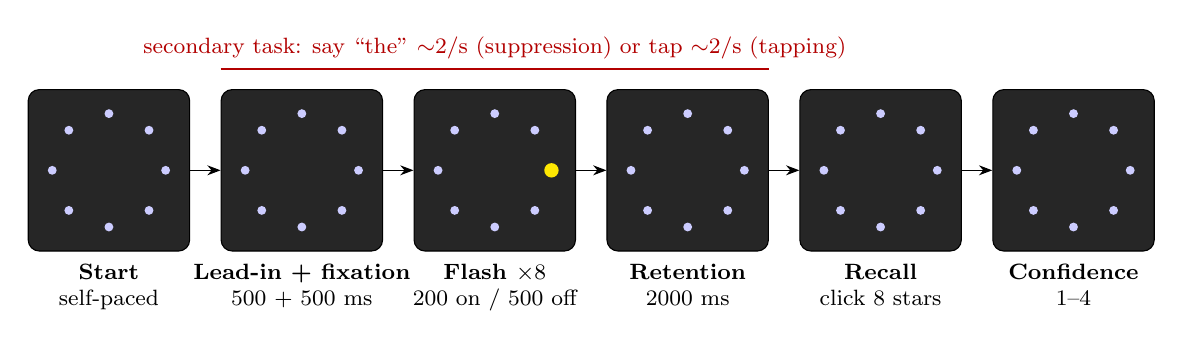
\begin{tikzpicture}[font=\footnotesize, box/.style={draw, rounded corners, minimum width=2.05cm, minimum height=2.05cm, fill=black!85}]
  \foreach \i/\lab/\dur in {0/Start/{self-paced}, 1/Lead-in + fixation/{500 + 500 ms}, 2/Flash $\times 8$/{200 on / 500 off}, 3/Retention/{2000 ms}, 4/Recall/{click 8 stars}, 5/Confidence/{1--4}} {
    \node[box] (b\i) at (\i*2.45,0) {};
    \node[below=1pt of b\i, align=center] {\textbf{\lab}\\\dur};
    \foreach \v in {0,...,7} { \fill[white!80!blue] ($(b\i.center)+({90-45*\v}:0.72)$) circle (1.6pt); }
  }
  \fill[yellow!90!orange] ($(b2.center)+(90-45*2:0.72)$) circle (2.6pt);
  \foreach \i in {0,...,4} { \draw[-{Stealth}] (b\i.east) -- (b\the\numexpr\i+1\relax.west); }
  \draw[thick, red!70!black] ($(b1.north west)+(0,0.25)$) -- node[above, align=center] {secondary task: say ``the'' $\sim$2/s (suppression) or tap $\sim$2/s (tapping)} ($(b3.north east)+(0,0.25)$);
\end{tikzpicture}
\caption{Trial structure. The secondary task (blocked: none / articulatory suppression / tapping) ran from the lead-in until the
end of retention. Recall: participants clicked the stars in the order they had lit up.}
\label{fig:trial}
\end{figure}

\subsection{Design and procedure}
Concurrent task was manipulated in three blocks (no load, articulatory suppression, tapping), with block order counterbalanced
across participants (all six orders). Each block began with instructions and one practice trial using a random permutation, followed by the
participant's four test sequences once each in random order (12 test trials in total). To keep a session to about 8--10
minutes, each participant saw four of the 14 sequences: \emph{repeat} ($K = 5$) and \emph{irregular} ($K = 16$), plus one
of six pairs (Table~\ref{tab:stimuli}), with pair and block order crossed across participants in a Latin square. Each pair
holds a chunked sequence with $K = 7$--8 and a harder sequence with $K = 9$--14, so every participant's sequences span the
whole complexity range (set means $K = 9.5$--10.5) and include at least one chunked sequence, and all 14 sequences are used
across the sample. Because the two anchors fix the ends of the complexity range, four sequences estimate a participant's
complexity slope almost as precisely as five did in simulations of the generative model, which gave similar (and low,
about 16--17\%) power for the suppression-vs-tapping contrast at $N = 24$ with four or five sequences per block. In practice the
six pairs were used by 6, 3, 6, 2, 5 and 1 participants and the six block orders by 2--8 participants each, because
participants chose their own link. Participants saw the same four sequences in all three blocks, so conditions were compared on identical material
within each participant. Sequences a
participant did not see are missing by design; the Bayesian mixed model handles this through its random intercepts for
sequences. On each
trial the participant pressed Start and began the secondary task; after a 1000-ms lead-in, whose last 500~ms showed a
central fixation cross, the eight locations flashed for 200 ms
each with a 700-ms stimulus-onset asynchrony (the timing of the behavioural training in \citealp{alroumi2021mental}), followed by
a 2000-ms retention interval. The requested speaking/tapping rate ($\sim$2 per second) differed from the flash rate (1.43 per
second), so the secondary task could not serve as a metronome for the sequence. The
participant then stopped the secondary task, clicked the stars in order (with an undo option), and rated their confidence
(1 = guess, 4 = certain). Performance feedback (number of positions correct) appeared above the next trial's Start button.
After each block, participants
rated how mentally demanding the block had been (1--7; the mental-demand item of the NASA-TLX,
\citealp{hart1988development}), to check that suppression and tapping were similarly demanding. After the task, participants
answered strategy questions and the 12 items of the Internal Verbalization factor of the Internal Representations Questionnaire
(\citealp{roebuck2020internal}; 5-point scale; ``I rarely vocalize thoughts in my mind'' reverse-scored; score = item mean). Demographics (age,
gender, course and field, year, highest level of mathematics, number of languages, English as first language, sleep the previous
night, weekly video-gaming, input device) were collected before the task. A session was designed to take about 8--10 minutes.

\paragraph{Dry run.} Before data collection the authors dry-ran the task in its demonstration and test modes on laptops and
phones, ran scripted end-to-end sessions in a browser with the uploads disabled, and analysed simulated datasets of 24
participants generated from the hypothesised model (\texttt{analysis/simulate.py}) to check that every analysis and figure
worked. Problems found this way (session length, recall correction, the microphone check) were fixed before or early in data
collection; test and demonstration sessions were never analysed.

\paragraph{Verification of the secondary tasks.}
\emph{Articulatory suppression} was checked with the microphone, with echo cancellation, noise suppression and automatic
gain control disabled. Only the root-mean-square amplitude was computed, every 50 ms, locally in the browser, and no audio was
recorded or transmitted. A calibration at the start sampled loudness during 2.5~s of silence and 4~s of softly repeating
``the''. With $L_q$ the median and $P_q$ the 95th percentile of the silent samples, and $L_v$ the 90th percentile of the speaking
samples, the threshold was $\theta = \max\!\big(\sqrt{L_q L_v},\, 1.25\,P_q\big)$: halfway between room and voice on a decibel
scale, but always above the room's loudest moments. Calibration succeeded when $L_v > 1.25\,\theta$ and $L_v > 0.002$ (about
$-54$~dBFS). Otherwise participants could try again or choose another microphone. In the first sessions (25--26 November)
microphone access was optional, and \NNoMic{} participants declined or could not grant it; their suppression trials ran without
verification and were counted as valid. From 26 November microphone access was required: participants who blocked it were shown
how to allow it and could not continue without it, and every later participant completed the check. On each trial, compliance was the proportion
of 500-ms windows that contained at least one sample above $\theta$; trials with compliance $< .80$ were flagged. The longest
silent stretch on each trial was also logged, because loudness alone does not show that speech was continuous.
\emph{Tapping} (Space bar, or an on-screen pad on touch devices) was compliant when at least .80 of the 1-s windows contained a
tap and the mean rate was at least 1~Hz. Participants saw a live loudness/tap meter.

\subsection{Measures}
For each trial with sequence $s$ and response $r$, \emph{serial accuracy} was $\frac{1}{8}\sum_{i} [r_i = s_i]$; we also
recorded an order-tolerant similarity, $1 - \mathrm{Lev}(s,r)/8$, and the number of correct items before the first error.
For each participant and condition, the \emph{compression benefit} $\beta_c$ was the negative ordinary least-squares slope of
serial accuracy on LoT complexity (accuracy lost per complexity unit; larger = stronger compression). The
\emph{suppression-specific flattening} was $\beta_{\text{tap}} - \beta_{\text{AS}}$. The time of every recall click was recorded. For the seven sequences whose minimal program has explicit sub-programs
(2squares, 2arcs, 2rectangles: a boundary after item 4; 4segments, 4diagonals, 2crosses, alternate: boundaries after items 2,
4 and 6), \emph{boundary slowing} was the mean inter-click interval entering a new sub-program minus the mean interval within
one, using only clicks made before the first error, in trials answered without corrections \citep{tabbane2026humans}.
During recall, clicking a numbered star cleared its number, and the next star clicked took the lowest free number. \emph{Metacognitive sensitivity} in each
condition was the Spearman correlation between confidence and accuracy across trials \citep[cf.][]{fleming2014measure}.
Alternative complexity descriptors were computed from each canonical sequence's step sequence (step $=$ vertex difference
mod 8): Lempel--Ziv complexity \citep{lempel1976complexity}, Shannon entropy of steps, number of runs of identical steps, total
chord length, and number of path self-crossings.

\subsection{Exclusions and analysis}\label{sec:excl}
We excluded demonstration and test sessions and kept one session per email address (the first complete one). The planned
compliance rule removed dual-task trials with a non-compliant secondary task (\NInvalidTrials{} of the \NDualTrials{}
suppression and tapping trials) and participants with fewer than 50\% valid trials in either dual-task block. This rule
removed far more people than expected: \NExcluded{} of \NAll{}, of whom \NTapFail{} failed the tapping criterion and \NAsFail{}
the suppression criterion (\NBothFail{} both). Because the rule concerns only the dual-task blocks, we deviated from the plan
in one respect, decided before looking at any outcome: analyses that do not compare conditions (the no-load compression effect
H1, the complexity curve, the metric comparison, the practice and effort checks and the individual-difference analyses of
no-load performance) use all \NAll{} participants, while every comparison between suppression and tapping uses the
compliant sample ($N = \NFinal$) and is repeated with all \NAll{} participants and no compliance filter as a sensitivity
analysis. H1 was tested with a one-sample $t$-test of $\beta_{\text{none}}$ against zero. Conditions were
compared with repeated-measures ANOVAs (Greenhouse--Geisser corrected; \citealp{greenhouse1959methods}) on accuracy and on
$\beta$, followed by planned paired contrasts reported with $d_z$ and default JZS Bayes factors (\citealp{rouder2009bayesian};
BF$_{10} > 3$ = evidence for a difference, $< 1/3$ = evidence for no difference). For item-level analyses that do not
reduce each person to a slope, we fitted (i) a Bayesian logistic mixed model (variational Bayes) with random intercepts for
participants and sequences and random complexity slopes for participants, with round number (1 to 3) as a covariate to
absorb practice effects. This is the richest random-effects structure our
software supports, short of the maximal structure recommended by \citet{barr2013random}. We also fitted (ii) a logistic generalised estimating equation \citep{liang1986longitudinal} to the
correctness of each serial position, with centred complexity $\times$ condition (reference: tapping) and an exchangeable working
correlation within participants. Complexity metrics were compared by the AIC of binomial GLMs with participant fixed effects
(lower = better). Individual-difference analyses were exploratory: Pearson and Spearman correlations with Holm correction, and
Welch $t$-tests with Hedges' $g$. Robustness checks repeated the key contrast with order-tolerant Damerau--Levenshtein scoring, without the compliance
filter, and with a strict filter that also removed suppression trials containing a silent stretch longer than 1~s. Error bars
show within-subject 95\% intervals \citep{cousineau2005confidence,morey2008confidence}.

% =====================================================================
\section{Results}

\subsection{H1: compression}
Accuracy fell steeply with LoT complexity (Fig.~\ref{fig:curve}). With no concurrent task, the compression benefit was reliably
positive, $\beta_{\text{none}} = \HoneM$ per complexity unit, \HoneStat. Clicks also slowed when participants entered a new
sub-program (H1b): boundary slowing, pooled over the three blocks because each participant saw only one or two
chunked sequences per block, was positive on average but not reliable, \HoneBoundary; only participants who answered
chunked sequences without corrections contribute to this measure. Overall accuracy dropped from \AccKFive{} for the simplest
sequence ($K = 5$) to \AccKSixteen{} for the most complex ($K = 16$). In the metric comparison (Table~\ref{tab:metrics}),
LoT complexity predicted recall better than Lempel--Ziv complexity, step entropy and path crossings, but the simplest
descriptor, the number of runs of identical steps, fitted best ($\Delta\text{AIC}_{\text{LoT}} = \LoTdAIC$). Because each
participant saw only four of the 14 sequences and the descriptors are strongly correlated across so few sequences, this
comparison is weak evidence; it does not show that LoT complexity is the right measure, only that recall tracks
regularity of several kinds.

\begin{figure}[t]\centering
\includegraphics[width=.62\linewidth]{fig_curve.pdf}
\caption{Serial recall accuracy as a function of LoT complexity in each condition, all \NAll{} participants and all trials
(points: sequence means with within-subject SE; lines: least-squares fits). Sequences seen by few participants have wide or
no error bars.}\label{fig:curve}
\end{figure}

\input{../analysis/out/tables/metrics.tex}

\subsection{H2: does suppressing inner speech remove the compression advantage?}
In the compliant sample ($N = \NFinal$), overall accuracy did not differ reliably between conditions, \AccAov{} (no load:
$M = \AccNone$; suppression: $M = \AccAs$; tapping: $M = \AccTap$), and the verbal-specific cost (tapping vs.\ suppression)
was not significant, \HtwoCostAsTap. The compression benefit did not differ between conditions, \SlopeAov. Suppression did not
flatten it relative to tapping; if anything the slope was steeper under suppression ($\beta_{\text{AS}} = \CompressAs$,
$\beta_{\text{tap}} = \CompressTap$), \HtwoAsTap{} (Fig.~\ref{fig:paired}b; Table~\ref{tab:tests}). The Bayes factor slightly
favours no difference but is far from conclusive. The item-level Bayesian model (Table~\ref{tab:glmm}) agreed that the
complexity $\times$ suppression interaction was uncertain (its 95\% interval includes zero); it estimated lower accuracy under
suppression than tapping at average complexity and a steeper complexity effect with no load than with tapping. The GEE
(Table~\ref{tab:gee}), with only \NFinal{} clusters, found no reliable effects. The null result held with Damerau--Levenshtein
scoring (\HtwoAsTapDL) and with the strict continuity filter (\HtwoAsTapStrict).

The sensitivity analysis with all \NAll{} participants and no compliance filter pointed the other way: the slope was flatter
under suppression ($\beta_{\text{AS}} = \CompressAsAll$) than under tapping ($\beta_{\text{tap}} = \CompressTapAll$), the
pattern H2b predicts, but not significantly, \HtwoAsTapUnfiltered{} (BF$_{10} \approx 1$: the data do not discriminate). The
curves in Fig.~\ref{fig:curve} show this flatter suppression line. Overall accuracy did not differ between suppression and
tapping in the full sample either, \HtwoCostAsTapAll. Boundary slowing could not be compared between conditions
(\HtwoBoundaryAsTap).

Manipulation and practice checks (all participants): suppression was rated more mentally demanding than no load,
\CheckEffortAsNone, but not more demanding than tapping, \CheckEffortAsTap, so the two dual tasks were roughly matched in
felt effort. Accuracy did not change from the first to the third round, \CheckPractice, so practice did not confound the
counterbalanced condition effects.

\begin{figure}[t]\centering
\begin{subfigure}{.32\linewidth}\includegraphics[width=\linewidth]{fig_accuracy.pdf}\caption{}\end{subfigure}
\begin{subfigure}{.32\linewidth}\includegraphics[width=\linewidth]{fig_compression.pdf}\caption{}\end{subfigure}
\begin{subfigure}{.32\linewidth}\includegraphics[width=\linewidth]{fig_meta.pdf}\caption{}\end{subfigure}
\caption{Compliant sample ($N = \NFinal$): (a) mean accuracy, (b) compression benefit and (c) metacognitive sensitivity per
condition. Grey lines: individual participants; coloured points: means with 95\% CI. Metacognitive sensitivity cannot be
computed for a person whose four confidence ratings or accuracies in a block are all equal.}\label{fig:paired}
\end{figure}

\input{../analysis/out/tables/tests.tex}
\input{../analysis/out/tables/glmm.tex}
\input{../analysis/out/tables/gee.tex}

\subsection{H3: metacognition and individual differences}
Metacognitive sensitivity could be estimated in both dual-task blocks for only three compliant participants (a Spearman
correlation over four trials is undefined when all ratings or all scores are equal), so the suppression-vs-tapping contrast
(\HthreeMetaAsTap) is not interpretable.

\paragraph{Age and other individual differences.} No individual-difference correlation was significant, before or after Holm
correction (Table~\ref{tab:corr}; Fig.~\ref{fig:indiv}). Age was unrelated to no-load accuracy ($r = -.02$) and to the
compression benefit ($r = .21$). The age range was narrow apart from four participants (14, 14, 15 and 68 years), so these
correlations rest mostly on those four people; Spearman correlations with age, which are less sensitive to them, were also
small ($|\rho| \leq .29$). The largest association was a negative one between the number of languages spoken and no-load
accuracy (Pearson $r = -.29$, not significant; Spearman $\rho = -.48$); as one of eight exploratory tests we do not interpret it. Mathematical training, sleep, video-gaming and
habitual inner speech (IRQ; compliant sample only, $n = \NFinal$) were also unrelated to performance. Women ($n = 5$) and men
($n = 17$) did not differ in accuracy or compression benefit (Table~\ref{tab:groups}); a STEM vs.\ non-STEM comparison was not
possible because only \NNonStem{} participants studied a non-STEM subject. After the task, every participant reported noticing
that some sequences formed patterns; most described their strategy as remembering the shape (11) or the positions (5) or the
motion (4), and only two said they used words.

\IfFileExists{../analysis/out/tables/corr.tex}{\input{../analysis/out/tables/corr.tex}}{}
\IfFileExists{../analysis/out/tables/groups.tex}{\input{../analysis/out/tables/groups.tex}}{}

\begin{figure}[t]\centering
\includegraphics[width=.48\linewidth]{fig_serial.pdf}\hfill
\includegraphics[width=.48\linewidth]{fig_metrics.pdf}
\caption{Left: serial-position curves. Right: $\Delta$AIC of each complexity metric (lower = better fit).}\label{fig:serial}
\end{figure}

\begin{figure}[t]\centering
\includegraphics[width=\linewidth]{fig_individual.pdf}
\caption{Exploratory individual differences: no-load accuracy and compression benefit against age and mathematical training
(all participants), and suppression-specific flattening against habitual inner speech (compliant sample).}\label{fig:indiv}
\end{figure}

% =====================================================================
\section{Discussion}
\paragraph{Compression replicates in a recall task.} With no concurrent task, sequences with a shorter description were recalled
far better than complex ones, with a very large effect ($d_z = 1.47$) in a short, eight-minute online session. This replicates
the central finding of the octagon paradigm \citep{amalric2017language,alroumi2021mental} in a new format: free serial recall
by clicking, with random rotations and reflections so that participants could not memorise absolute positions. The effect was
present in 22 of the \NAll{} participants (a positive no-load slope), and it did not depend on practice. Inter-click intervals tended to lengthen at the boundaries of the
minimal program, as \citet{tabbane2026humans} reported, but the effect was not reliable here, plausibly because each participant
contributed only a few error-free chunked trials. LoT complexity was a good but not the best predictor of recall: with only 14
sequences, and four per person, simple descriptors such as the number of runs of identical steps are almost interchangeable
with LoT complexity, and a larger stimulus set is needed to tell them apart.

\paragraph{Does compression need inner speech?} The answer from this study is: we cannot tell yet. In the participants who
did both concurrent tasks properly, articulatory suppression did not remove the compression benefit, the result a
non-linguistic geometric code predicts \citep{dehaene2022symbols,fedorenko2024language} and the result earlier work on
spatial memory under suppression would lead one to expect \citep{vandierendonck2004working,rossiarnaud2006symmetry}. But that
sample had only \NFinal{} people. With everyone included, suppression flattened the slope somewhat, the pattern a verbal
recoding account predicts \citep{lupyan2012linguistically}, yet that analysis includes trials in which people were not
doing the concurrent task, and it was not significant. Neither result is strong evidence, and the Bayes factors near 1 say
so explicitly. The participants' own reports lean towards a non-verbal code: only two of \NAll{} said they used words, while
most remembered shapes, positions or motion, consistent with spontaneous but not dominant verbal labelling of spatial material
\citep{seabra2025verbal}.

\paragraph{Individual differences.} Memory for the sequences was unrelated to age, gender, mathematical training, sleep,
gaming and inner-speech habits. With $N = \NAll$ only large correlations ($|r| \gtrsim .55$) could be detected, and the
sample was homogeneous: mostly male STEM undergraduates aged 18--22. The absence of an age effect should therefore not
be read as evidence that age does not matter; it reflects the narrow age range.

\paragraph{Limitations.} (1) \emph{Compliance.} The main weakness is that \NTapFail{} of \NAll{} participants did not keep
tapping. Several tapped during the warm-up and then stopped completely, which suggests that the instruction was not clear
enough or that taps were sometimes not registered; the warm-up should have required a steady beat before the block could
start. Suppression compliance was better once the microphone check was compulsory, but some participants spoke too quietly
for the threshold. (2) \emph{Power.} The compliant sample could detect only very large effects ($d_z \geq \MinDz$), and even the
full sample could not detect the small-to-medium interaction that H2 concerns. (3) \emph{Design.} Each person saw four
sequences, four trials per condition, which makes per-person slopes and especially metacognition noisy; sequence pairs and
block orders were not evenly used. (4) \emph{Interpretation.} Suppression blocks subvocal rehearsal, not the whole language
network; tapping was single-key and non-spatial, so spatial interference was not tested; eye-movement rehearsal was not
controlled \citep{desardenberg2024inter}; simple shapes are also easy to name, which confounds compression with nameability
\citep{seabra2025verbal}; and the IRQ measures a habit, not the strategy used on this task. (5) \emph{Setting.} Sessions ran
unsupervised on participants' own devices, and the microphone check was not validated against human observers.

\paragraph{Next steps.} A follow-up should enforce the concurrent tasks (a warm-up that must be passed, live feedback, and
supervised sessions), test 50--60 people to detect a medium-sized interaction, give each person more sequences, add a spatial-tapping
arm to separate verbal from visuospatial interference, and use supraspan sequences to avoid ceiling effects
\citep{tabbane2026humans}.

\paragraph{Conclusion.} Constellations, a short browser-based task, reproduces the language-of-thought compression effect in
spatial sequence memory with a large effect in \NAll{} people. Whether that compression depends on inner speech remains open:
the compliant sample showed no sign of it and the full sample a weak, non-significant trend, so a larger, better-controlled
study is needed.

\section*{Data and code availability}
The task runs at \url{https://constellations-task.vercel.app}; its code (\texttt{task/}), the analysis pipeline
(\texttt{analysis/analyze.py}) and this report's source are at \url{https://github.com/mahir-m01/constellations}. The data
(one file per participant, and an Excel workbook with all participants and trials) are provided with the submission. Because
they contain participants' email addresses, they go only to the instructor and are never part of the public code repository.
All statistics, tables and figures in this document are generated from the data by the analysis script.

\bibliographystyle{apalike}
\bibliography{refs}
\end{document}
